%!TEX root = ../dokumentation.tex

\chapter{Die Architektur und Funktionalität von Schachcomputern}

\section{Einleitung}

\subsection{Die Entwicklung von Schachcomputern}
Die Geschichte der Schachcomputer zeigt die Entwicklung von künstlicher Intelligenz und Rechenleistung. 
In den 1940er Jahren wurden einige der frühesten theoretischen Arbeiten zu Schachspielcomputern von Informatikern 
wie Claude Shannon und Alan Turing unternommen. Trotz der begrenzten Rechenressourcen, die ihnen zur Verfügung standen, 
erkannten sie das Potenzial von Computern, sich in einem Spiel wie Schach zu behaupten.~\cite{History_of_chess_engines_2023_wikipedia}

Die ersten tatsächlichen Schachspielcomputer wurden jedoch erst in den 1960er und 1970er Jahren geschaffen. Diese Maschinen, 
wie das Schachspielcomputersystem von IBM namens Deep Blue, konnten auf dem Niveau eines kompetenten Menschen spielen, 
waren aber weit entfernt von der Weltklasse.

Erst mit dem Aufkommen leistungsstarker Computer und besseren Algorithmen im späten 20. und frühen 21. Jahrhundert 
waren Computer in der Lage, mit menschlichen Weltmeistern zu konkurrieren und diese zu schlagen. 
1997 machte IBMs Deep Blue weltweit Schlagzeilen, als es den amtierenden Schachweltmeister Garry Kasparow in einem Sechsspiel-Match besiegte.~\cite{Chris_Higgins_2017_mentalfloss}


Seitdem hat die Leistungsfähigkeit von Schachcomputern nur noch zugenommen, wobei Programme wie Stockfish und Komodo selbst die stärksten 
menschlichen Spieler übertreffen. Und in den letzten Jahren wurde Aufstieg des maschinellen Lernens im Schach gesehen, 
wobei das AlphaZero-Programm von Google sich selbst trainiert, um in nur wenigen Spielstunden ein Weltklassespieler zu werden.~\cite{History_of_chess_engines_2023_wikipedia}

\subsection{Rolle und Zweck von Schachcomputern}
Der Zweck von Schachcomputern geht über das einfache Gewinnen von Spielen hinaus. Auf einer grundlegenden Ebene besteht das Ziel eines Schachcomputers darin, 
menschenähnliches Denken und Entscheiden im Kontext des Spiels zu simulieren. Schachcomputer dienen daher als Plattform zur Erforschung komplexer Konzepte 
in der künstlichen Intelligenz, einschließlich Suchalgorithmen, Mustererkennung und strategischer Planung.

Darüber hinaus bieten Schachcomputer praktische Anwendungen. Sie dienen menschlichen Spielern als wertvolle Werkzeuge, indem sie hochrangige Übungsgegner 
bereitstellen und eine detaillierte Analyse von Spielen anbieten. Schachcomputer stellen ebenfalls eine Hilfe für neue Spieler dar, indem sie durch
detaillierte Analysen der Spiele die Schwächen eines Spielers individuell zu erkennen und den Nutzer darauf aufmerksam machen. 
Ein Beispiel dafür ist die Spielanalyse von Chess.com, bei der ein virtueller Coach nochmal über das Spiel mit dem Nutzer geht und ihm Tipps gibt.

Mit Blick auf die Zukunft ist es wahrscheinlich, dass Schachcomputer eine bedeutende Rolle in der weiteren Entwicklung spielen werden, 
da das Feld der künstlichen Intelligenz sich weiterhin entwickelt.~\cite{Larry_Greenemeier_2017_scientificamerican}

\section{Schachcomputer ohne maschinelles Lernen}

\subsection{Definition}
Schachcomputer ohne maschinelles Lernen, auch als traditionelle Schach-Engines bekannt und stellen eine Klasse von künstlichen Intelligenzprogrammen dar, 
die entwickelt wurden, um Schach zu spielen. Im Gegensatz zu Bots, die auf maschinellem Lernen basieren, lernen diese Engines nicht aus ihren Erfahrungen, 
sondern folgen einem vordefinierten Satz von Regeln und Algorithmen.
Sie nutzen deterministische und heuristische Methoden, um den Spielzustand zu bewerten und den optimalen Zug zu bestimmen.

Traditionelle Schachcomputer waren jahrzehntelang der Mainstream. Die erfolgreichsten Beispiele, wie Stockfish und Komodo, 
wurden durch viele Iterationen und Verbesserungen entwickelt und können auf einem Niveau weit über den menschlichen Fähigkeiten spielen.
Sie wenden dabei eine Vielzahl von Techniken an, um den Zustand des Spiels zu verarbeiten und zu analysieren.

\subsection{Positionsbewertung}
Die Positionsbewertung spielt eine entscheidende Komponente, die es Schachcomputern ermöglicht, die Stärke und das strategische Potenzial eines bestimmten 
Spielzustands einzuschätzen. Dieser Prozess beinhaltet die Analyse der Anordnung der Figuren und die Zuweisung eines numerischen Werts zu dieser 
Konfiguration auf der Grundlage einer Vielzahl von Kriterien.

\subsubsection{Materialgleichgewicht}
Die grundlegendste Bewertungsmethode besteht darin, den Gesamtwert der Figuren auf dem Brett für beide Seiten zu zählen. 
Jeder Figur wird ein bestimmter Wert zugewiesen (Dame: 9, Turm: 5, Läufer: 3, Springer: 3, Bauer: 1), 
und das Materialgleichgewicht ist die Differenz zwischen den beiden Seiten. Die Seite mit dem höheren Gesamtwert steht im Allgemeinen besser da.

\subsubsection{Aktivität der Figuren}
Aktive Figuren sind im Allgemeinen wertvoller als passive. Ein Springer beispielsweise, der sich in der Mitte des Bretts befindet, 
könnte potenziell acht verschiedene Felder angreifen oder darauf ziehen, während ein Springer in einer Ecke nur auf zwei Felder ziehen könnte. 
Eine Bewertungsfunktion würde dem zentraler gelegenen Springer einen höheren Wert geben.
Für jede Figur kann also eine Map angelegt werden, welche die favorisierten Felder höher gewichtet.

\begin{figure}[ht]
    \centering
    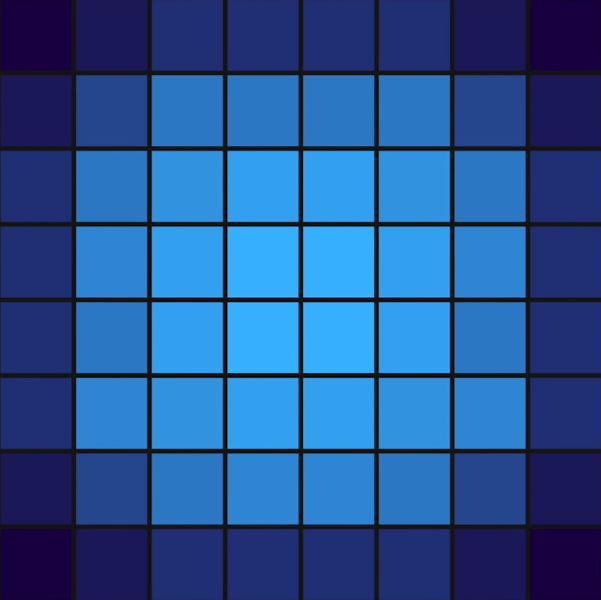
\includegraphics[scale=0.3]{images/knight_map.png}
    \caption{Springer Map}
\end{figure}

Die Abbildung 4.1 zeigt eine Beispielhafte Map für den Springer. Je heller der Blauton ist, desto höher wird das jeweilige Feld gewertet.~\cite{Lague_Sebastian_2021_youtube}

\subsubsection{Kontrolle des Zentrums}
Die Kontrolle des Zentrums ist im Allgemeinen vorteilhaft, da sie mehr Mobilität für die Figuren des Spielers 
bietet und die Position des Gegners einschränken kann.

\subsubsection{Kontrolle der Felder}
Felder, die von einem Spieler kontrolliert werden und die dieser angreift oder verteidigt, sind wertvoll, insbesondere wenn sie im Zentrum oder
im gegnerischen Spielraum liegen.

\subsubsection{Königssicherheit}
Die Sicherheit des Königs ist ein weiterer wichtiger Faktor. Ein Spieler, dessen König möglichen Schachmatt-Drohungen ausgesetzt ist, 
steht im Nachteil. Deshalb berücksichtigen Bewertungsfunktionen Faktoren wie die Frage, ob der König von Bauern geschützt ist oder
ob der Gegner viele Figuren in der Nähe des Königs hat.

\subsubsection{Bauernstruktur}
Trotz ihrer geringen Punktewertung können Bauern und ihre Struktur einen großen Einfluss auf das Spiel haben. 
Bauernketten, doppelte Bauern, isolierte Bauern, durchgebrochene Bauern sind alles wichtige Faktoren bei der Positionsbewertung. 
Im Allgemeinen werden starke Bauernstrukturen bevorzugt vor allem im weiteren Spielverlauf.

\subsection{Suchtechniken}
Suchtechniken sind das Kernstück des Entscheidungsprozesses eines Schachcomputers. Techniken wie Minimax-Suche, werden verwendet, um den Spielbaum zu erkunden, 
der die zukünftigen Möglichkeiten im Spiel repräsentiert. Die Idee besteht darin, das Worst-Case-Szenario zu minimieren, 
unter der Annahme eines optimalen Spiels des Gegners.

\begin{figure}[ht]
    \centering
    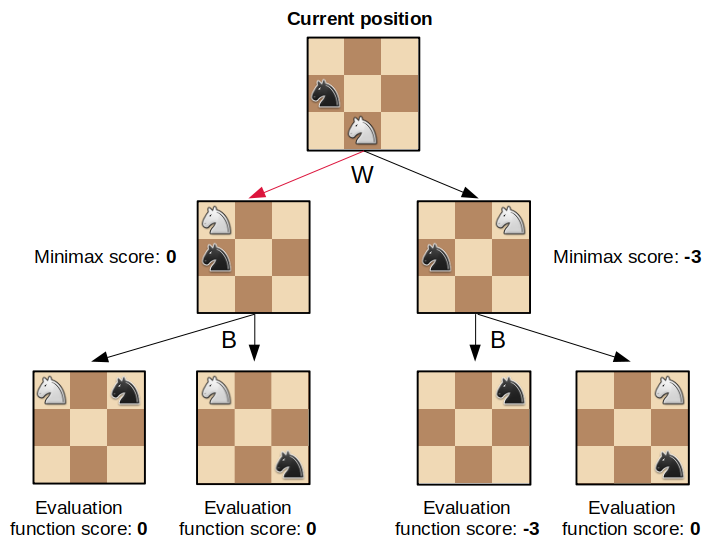
\includegraphics[scale=0.3]{images/chess_minimax_position.png}
    \caption{Minimax Algorithmus}
\end{figure}

Dabei wird der Suchbaum bis zur untersten Stufe durchgelaufen und die Endposition evaluiert. In Abbildung 4.1 ist die Evaluation für den Fall unten links
0. Diese Evaluation wird dann anschließend mit den anderen möglichen Ausgängen aus der vorherigen Position verglichen. Nun wird zwischen weißem und schwarzem 
Spieler unterschieden. Weiß stellt dabei den zu maximierenden Spieler und schwarz den zu minimierenden Spieler dar. Das heißt, dass 
der weiße Spieler eine Position mit einer möglichst hohen Evaluationszahl erlangen will und umgekehrt. Der beste Ausgang wird dann an die darüberliegende Ebene 
übertragen. Dieses Prozedere wird bis zur obersten Ebene wiederholt, sodass der Computer dann den Zug spielt, der für ihn das beste Ergebnis, unter 
Annahme des perfekten Spiels des Gegners.~\cite{Diderich2001}

\subsection{Alpha-Beta-Pruning}
Alpha-Beta-Pruning ist eine bedeutende Verbesserung des Minimax-Algorithmus, der in Entscheidungsfindung und Spieltheorie verwendet wird. 
Dieser Suchalgorithmus wird hauptsächlich in Spielen eingesetzt, in denen die Spieler abwechselnd ziehen. 
Sein Zweck ist es, die Anzahl der vom Minimax-Algorithmus ausgewerteten Knoten zu reduzieren, wodurch die Effizienz erhöht wird.

Obwohl der Minimax-Algorithmus konzeptionell einfach und effektiv ist, ist er auch rechenintensiv, insbesondere für Spiele mit großen Entscheidungsbäumen wie Schach. 
Der Algorithmus muss alle Knoten des Baumes durchlaufen, um eine Entscheidung zu treffen, was bei großen Suchräumen sehr ineffektiv ist.

Alpha-Beta-Pruning bietet eine Lösung für dieses Problem. Es handelt sich um eine Optimierungsmethode, die die Anzahl der vom Minimax-Algorithmus 
zu bewertenden Knoten erheblich reduziert. Es funktioniert, indem es Zweige im Spielbaum eliminiert, 
die nicht durchsucht werden müssen, weil bereits ein besserer Zug verfügbar ist.

Dieser Algorithmus hält für jeden Knoten im Spielbaum zwei Werte, Alpha und Beta, fest. Alpha repräsentiert die minimale Punktzahl, 
die der maximierende Spieler sicher hat, während Beta die maximale Punktzahl darstellt, die der minimierende Spieler sicher hat. 
Während der Suche, wenn der maximierende Spieler eine höhere oder gleich hohe Punktzahl (durch ein Kind des Knotens) findet als Beta, kann er aufhören, 
die anderen Kinder des Knotens zu betrachten, weil der minimierende Spieler niemals zulassen wird, dass das Spiel diesen Knoten erreicht. 
Ebenso kann der minimierende Spieler aufhören zu suchen, wenn er eine Punktzahl findet, die niedriger oder gleich Alpha ist, 
weil der maximierende Spieler niemals zulassen wird, dass das Spiel diesen Knoten erreicht.
\begin{figure}[ht]
    \centering
    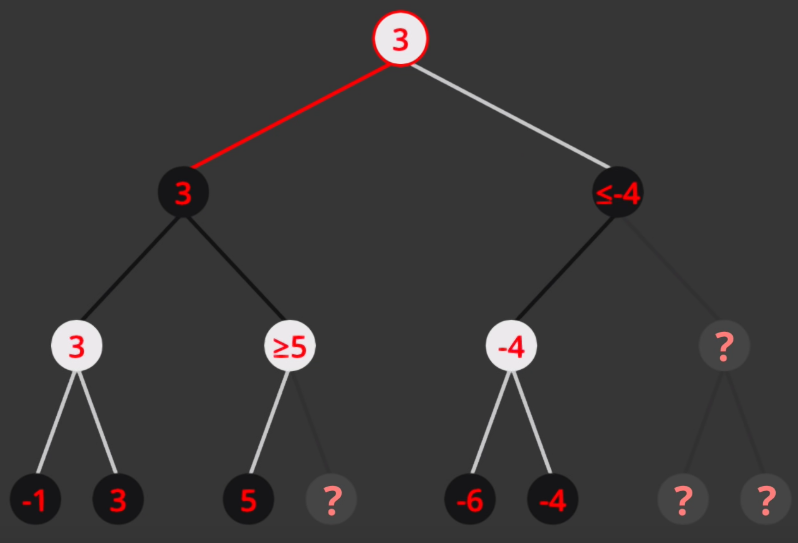
\includegraphics[scale=0.5]{images/alpha-beta-pruning.png}
    \caption{Alpha-Beta-Pruning}
\end{figure}

Auf diese Weise ermöglicht Alpha-Beta-Pruning dem Minimax-Algorithmus, mehr Knoten zu prüfen, 
die wahrscheinlich die endgültige Entscheidung beeinflussen, und Knoten zu verwerfen, die das nicht tun. 
In der Abbildung 4.2 sind die verworfenen Knotenpunkte mit Fragezeichen gekennzeichnet.
Dies macht den Suchalgorithmus weitaus effizienter und ermöglicht es ihm, tiefer in den Spielbaum vorzudringen, was wiederum die KI stärker macht.

Alpha-Beta-Pruning hat keinen Einfluss auf das endgültige Ergebnis des Minimax-Algorithmus. Der Algorithmus macht die Berechnung nur schneller. 
Er ermöglicht es, Zweige, die keinen Einfluss auf die endgültige Entscheidung haben, zu verwerfen und dadurch Rechenressourcen und Zeit zu sparen. 
Für Spiele wie Schach ist es eine notwendige Verbesserung um den Computer in Echtzeit spielen zu lassen.

Jedoch hängt die Effizienz und gesparte Zeit stark davon ab, in welcher Reihenfolge die Züge durchprobiert werden.~\cite{Aayush_Parashar_2023_springer}

\subsection{Zugsortierung}  
Das Ziel der Zugsortierung in Schach-Engines besteht darin, die Effizienz des Suchalgorithmus zu verbessern.
Durch die zuerst erfolgende Untersuchung vielversprechender Züge kann die Schach-Engine schneller einen Cut-Off in ihrem Suchbaum erreichen. 
Cut-Offs treten im Minimax-Algorithmus mit Alpha-Beta-Pruning auf, wenn die Engine feststellt, dass sie bereits einen besseren Zug gefunden hat als den, 
den sie gerade in Betracht zieht, sodass sie aufhören kann, den aktuellen Zug weiter zu analysieren.
Es wird hier zwischen verschiedenen Klassen an Zügen unterschieden.~\cite{Move_Ordering_2023_chessprogramming}

\subsubsection{Schlagzüge}
Züge, die ein gegnerisches Stück schlagen, werden in der Regel zuerst untersucht, da sie die Bewertung der 
Stellung signifikant verändern können.~\cite{Move_Ordering_2023_chessprogramming}

\subsubsection{Killerzüge}
Killerzüge sind Züge, die keine Schlagzüge sind, aber in einem Geschwisterknoten im Suchbaum auf der gleichen Tiefe einen Cut-Off verursacht haben. 
Diese Züge werden gespeichert und frühzeitig ausprobiert, wenn andere Knoten auf der gleichen Tiefe im Suchbaum analysiert werden.~\cite{Move_Ordering_2023_chessprogramming}

\subsubsection{Geschichts-Heuristik}
Diese Heuristik gibt Zügen, die in der Vergangenheit Cut-Offs verursacht haben, Priorität.
Sie basiert auf der Idee, dass, wenn ein Zug in einer Position gut war, er auch in einer anderen, aber ähnlichen Position gut sein könnte.~\cite{Move_Ordering_2023_chessprogramming}

\subsubsection{Gegen-Züge}
Der letzte Zug, der einen Cut-Off verursacht hat, wird für jedes Paar aus dem Zug des Gegners und dem eigenen Zug gespeichert.
Dies basiert auf der Idee, dass bestimmte Züge gute Antworten auf bestimmte Züge des Gegners sind.~\cite{Move_Ordering_2023_chessprogramming}

\subsubsection{Hauptvarianten-Züge}
Bei iterativen Suchen wird der beste Zug aus der vorherigen Iteration zuerst in der nächsten Iteration ausprobiert.~\cite{Move_Ordering_2023_chessprogramming}

\subsection{Transpositionstabellen}
Im Bereich des Schach-Computings spielen Transpositionstabellen eine entscheidende Rolle, um den Entscheidungsprozess des Computers effizient zu gestalten. 
Transpositionstabellen sind im Wesentlichen eine Form von Caching, die der Bot nutzt, um die Bewertung von zuvor berechneten Positionen zu speichern. 
Die gespeicherten Bewertungen können später abgerufen werden, was die Notwendigkeit einer kostenintensiven Neuberechnung vermeidet 
und die Leistung der Engine erheblich verbessert.~\cite{Jos_W._H_1970_researchgate}

\subsubsection{Verständnis der Transpositionstabellen}
Transpositionstabellen basieren auf dem Konzept der Transpositionen im Schach. 
Eine Transposition tritt auf, wenn eine bestimmte Position durch mehr als eine Zugfolge erreicht wird. 
Viele verschiedene Partien können zu der gleichen Position führen, und das Erkennen dieser identischen Positionen ist der 
Schlüssel zur Optimierung des Entscheidungsprozesses einer Chess-Engine.~\cite{Jos_W._H_1970_researchgate}

\begin{figure}[ht]
    \centering
    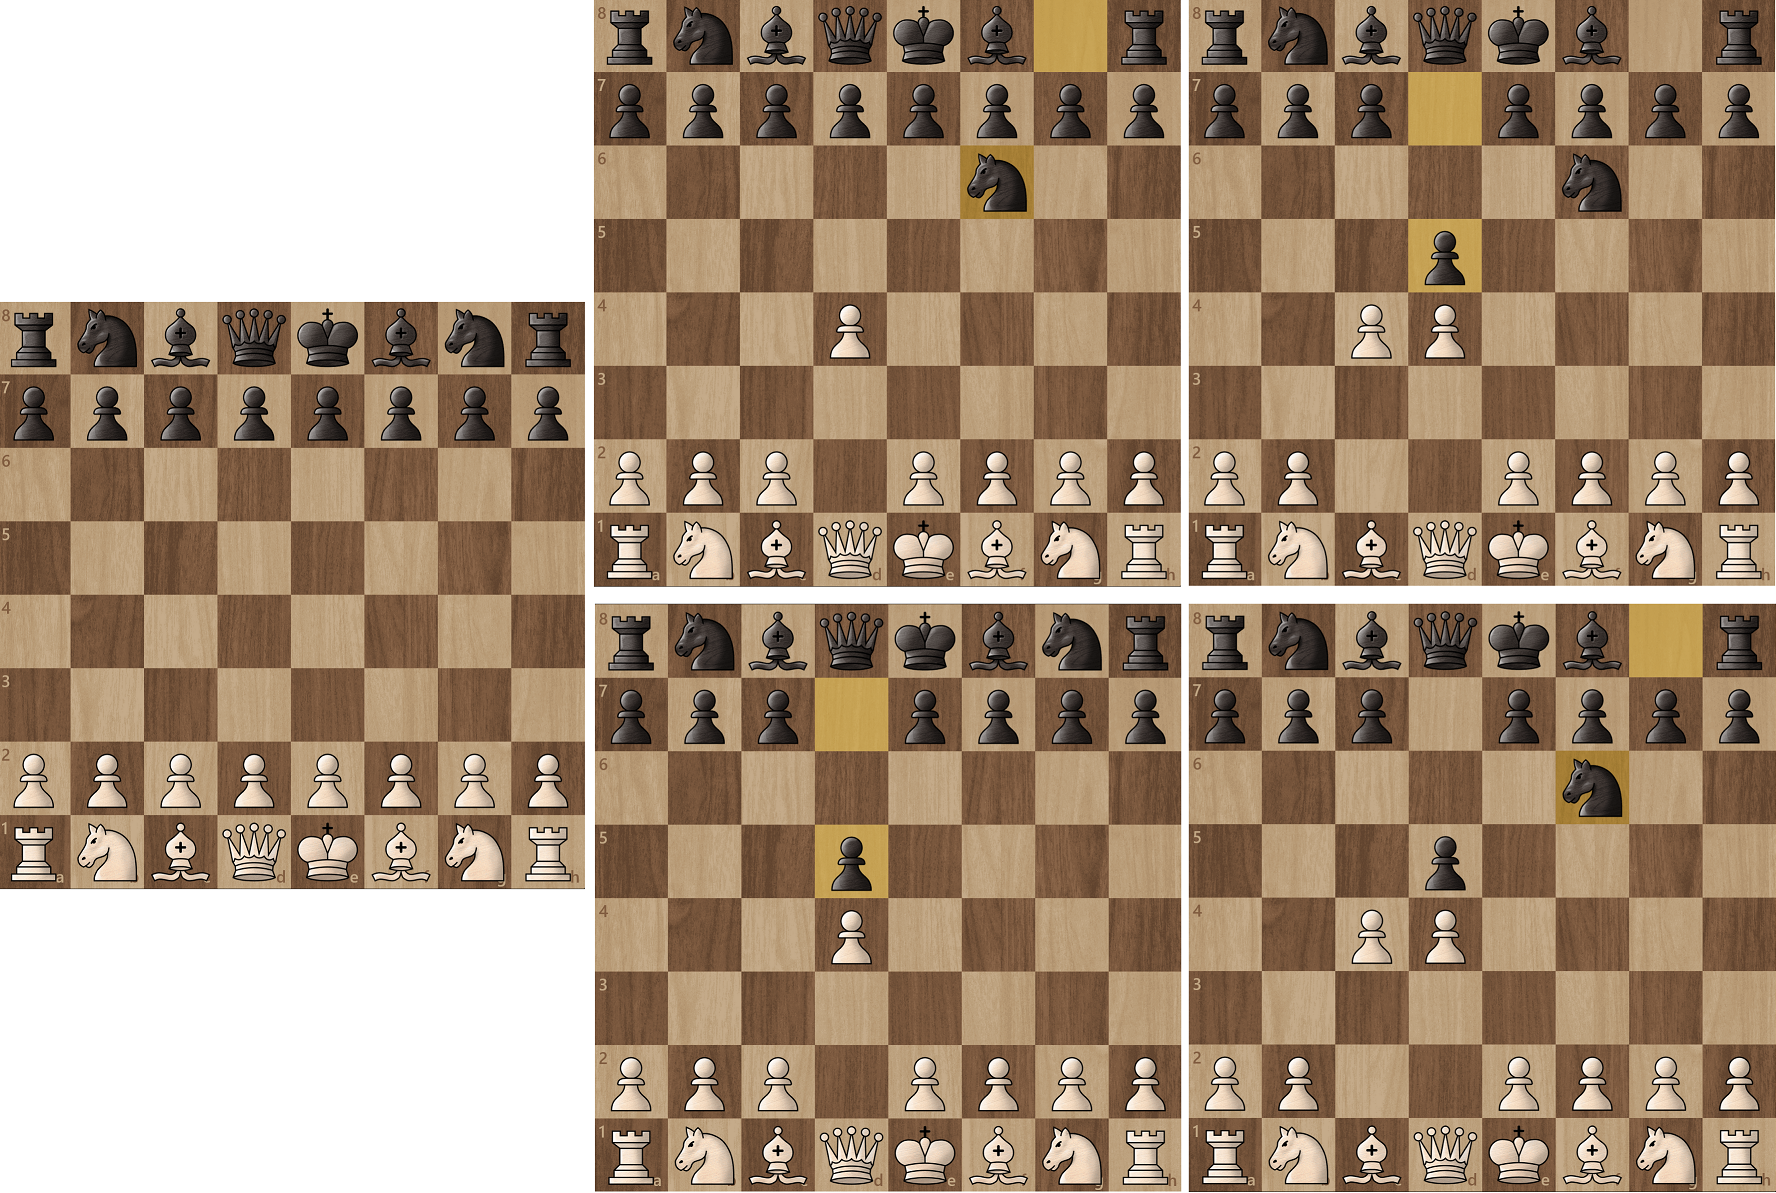
\includegraphics[scale=0.3]{images/transposition_example.png}
    \caption{Beispiel einer Transposition}
\end{figure}

Das Beispiel zeigt eine Stellung in einer Schacheröffnung. Trotz unterschiedlicher Reihenfolge der Züge des schwarzen Spielers, kommt es zur gleichen Endposition.
In komplexeren Stellungen kann diese Erkenntnis zu großen Zeitersparnissen führen.

Die Hauptidee hinter einer Transpositionstabelle ist, die Bewertung einer Position zu speichern, sobald sie berechnet wird. 
Die Bewertung zusammen mit der Position selbst wird in einer Tabelle gespeichert. 
Wenn später die gleiche oder eine transponierte Position auftritt, kann die Engine die Bewertung in der Transpositionstabelle nachschlagen, 
anstatt sie erneut zu berechnen.~\cite{Jos_W._H_1970_researchgate}

\subsubsection{Speicherung und Abfrage von zuvor berechneten Positionen}
Transpositionstabellen werden in Verbindung mit dem Suchalgorithmus des Computers verwendet. 
Wenn die Engine sich für den besten Zug entscheidet, durchsucht sie den Spielbaum, welcher eine Darstellung aller möglichen 
Zugsequenzen von der aktuellen Position aus ist. 
Wenn die Engine eine Position bewertet, überprüft sie zuerst, ob die Bewertung der Position in der Transpositionstabelle gespeichert ist. 
Falls ja, wird die gespeicherte Bewertung verwendet. Falls nicht, berechnet der Motor die Bewertung, 
speichert sie in der Tabelle und setzt dann die Suche fort.~\cite{Jos_W._H_1970_researchgate}

\subsection{Spielphasen}
Das Schachspiel wird in drei verschiedene Phasen unterteilt. Jede Phase hat dabei unterschiedliche Merkmale und Strategien, jedoch sind die Übergänge fließend.

\subsubsection{Eröffnung}
Die Eröffnungsphase des Spiels bezieht sich auf die anfänglichen Züge. Diese Phase ist entscheidend, um die Positionen der Spieler auf dem Brett zu etablieren, 
die Kontrolle über zentrale Felder zu gewinnen, den König in Sicherheit zu bringen und die Entwicklung der Figuren zu fördern. 
Es gibt zahlreiche gut dokumentierte Eröffnungsstrategien und Engines haben eine umfangreiche Bibliothek von Eröffnungszügen. 
Die Engine kann diese vorberechneten Züge verwenden, um sich durch die Eröffnungsphase zu navigieren, wodurch die Rechenzeit reduziert 
und ein starker Start gewährleistet wird.

\subsubsection{Mittelspiel}
Das Mittelspiel beginnt in der Regel, wenn die Spieler ihre anfängliche Figurenentwicklung abgeschlossen haben. 
Es ist gekennzeichnet durch dynamisches Spiel, bei dem strategische Planung, taktische Berechnungen und positionsbezogene Überlegungen eine wesentliche Rolle spielen. 
In dieser Phase führen die Computer eine umfassende Suche und Bewertung der möglichen Züge durch. 
Dieser Suchprozess beinhaltet oft Techniken wie Alpha-Beta-Pruning und die Verwendung von Transpositionstabellen, wie zuvor diskutiert. 
Die Entscheidungen, die in dieser Phase getroffen werden, beeinflussen die Spielrichtung erheblich und bereiten entweder einen entscheidenden Angriff 
oder ein ausgeglichenes Endspiel vor.

\subsubsection{Endspiel}
Die Endspielphase eines Schachspiels beginnt, wenn die meisten Figuren geschlagen wurden und überwiegend Könige und Bauern, zusammen mit wenigen anderen Figuren, 
auf dem Brett sind. Diese Phase ist in der Regel weniger taktisch als das Mittelspiel, beinhaltet aber komplexe strategische Überlegungen 
in Bezug auf Bauernstrukturen, Königsaktivitäten und Koordination der Figuren. 
Präzises Spiel ist in dieser Phase entscheidend, da ein Fehler das Ergebnis drastisch verändern kann. 
Engines nutzen Endspiel-Datenbanken, die perfekte Spielinformationen für alle Positionen mit einer geringen Anzahl von Figuren enthalten, 
um ein optimales Spiel in dieser Phase zu gewährleisten.

Jeder Spielphase hat unterschiedliche Herausforderungen, die von dem Computer gemeistert werden müssen. Die Eröffnung erfordert Kenntnisse der 
Eröffnungsprinzipien und eine umfangreiche Eröffnungsbibliothek, das Mittelspiel wird durch effiziente Suchalgorithmen und effektive Bewertungsfunktionen
entschieden und das Endspiel wird durch Endspiel-Datenbanken und spezielle Taktiken gewonnen.

\section{Schachcomputer auf Basis von maschinellem Lernen}

\subsection{Definition}
Schachcomputer, die auf maschinellem Lernen basieren, repräsentieren einen bedeutenden Fortschritt im Bereich der Schachinformatik. 
Diese Bots verwenden eine Reihe von Techniken des maschinellen Lernens, hauptsächlich das sogenannte Reinforcement Learning, 
um das Schachspiel zu verstehen und zu meistern. Im Gegensatz zu den traditionellen Engines stützen sich Schachcomputer, die auf maschinellem Lernen basieren, 
nicht ausschließlich auf handgemachte Evaluierungsfunktionen oder Algorithmen zur Zug-Generierung. 
Stattdessen lernen sie durch die Erfahrung des Spiels und optimieren ihre Strategien im Laufe der Zeit.~\cite{doi:10.1126/science.aar6404}

Ein prominentes Beispiel für einen Schachcomputer, der auf maschinellem Lernen basiert, ist DeepMinds AlphaZero, 
welches beispiellose Fähigkeiten im Bereich der Schach-KI zeigte. AlphaZero verwendet eine Variante der Monte Carlo Tree Search 
in Kombination mit tiefen neuronalen Netzwerken. Die neuronalen Netzwerke, die durch Selbstspiel und ohne Zugang zu existierendem Schachwissen trainiert wurden, 
leiten den Suchprozess, um vielversprechendere Züge zu erkunden. Mit der Zeit hat AlphaZero nicht nur alle traditionellen Schach-Engines übertroffen, 
sondern auch Strategien und Taktiken entdeckt, die neue Einblicke in das Spiel bieten.~\cite{David_Silver_2023_deepmind}

\subsection{Monte Carlo Tree Search}
Die Monte Carlo Tree Search ist eine suchbasierte KI-Methode, die in Spielen wird, bei denen der mögliche Zustandsraum enorm groß ist 
und daher eine vollständige Suche praktisch unmöglich ist. Die Monte Carlo Tree Search hat vier Hauptphasen: Auswahl, 
Expansion, Simulation und Rückwärtspropagation.~\cite{Ziad_Salloum_2019_towardsdatascience}

\subsubsection{Auswahl}
Startend an der aktuellen Spielposition navigiert der Algorithmus den Spielbaum unter Verwendung einer bestimmten Strategie, 
um den besten unterbewerteten Knoten zu finden.~\cite{Ziad_Salloum_2019_towardsdatascience}

\subsubsection{Expansion}
Sobald ein Knoten ausgewählt wurde, werden ein oder mehrere Kindknoten hinzugefügt, um mögliche Züge darzustellen.~\cite{Ziad_Salloum_2019_towardsdatascience}

\subsubsection{Simulation}
Vom expandierten Knoten aus wird eine zufällige Simulation des Spiels ausgeführt. Dies könnte so einfach sein wie das zufällige 
Spielen von Zügen bis zum Ende des Spiels.~\cite{Ziad_Salloum_2019_towardsdatascience}

\subsubsection{Rückwärtspropagation}
Nach der Simulation wird das Ergebnis auf alle Knoten in dem Pfad vom ausgewählten Knoten zurück zur Wurzel gegeben.

Dieser Prozess wird dann iterativ fortgesetzt, wobei jeder Durchlauf eine Suche darstellt, bis eine vordefinierte Bedingung erreicht ist, 
wie z.B. eine bestimmte Anzahl von Durchläufen, eine bestimmte Zeitgrenze oder eine ausreichende Gewissheit über den besten Zug.

Eine der Stärken vom \ac{MCTS} ist, dass er nicht auf heuristische Bewertungen der Spielpositionen angewiesen ist, 
wie es bei traditionellen suchbasierten Algorithmen der Fall ist. Stattdessen basiert \ac{MCTS} auf statistischen Analysen von simulierten Spielen, 
was dazu führt, dass sie oft unkonventionelle oder kreative Spielstrategien findet. Außerdem kann \ac{MCTS} auch in Spielen mit hohen 
Verzweigungsfaktoren effektiv eingesetzt werden, da sie durch die Verwendung von Simulationen die Notwendigkeit, 
den gesamten Spielbaum zu analysieren, umgeht.~\cite{Ziad_Salloum_2019_towardsdatascience}

\subsection{Übergang von nicht-maschinellem Lernen zu Schachcomputern auf Basis von maschinellem Lernen}
Der Übergang von Schachcomputern, die nicht auf maschinellem Lernen basieren, zu solchen, die es tun, 
markiert eine entscheidende Veränderung in der Herangehensweise an die Schachinformatik. 
Traditionell wurden Schachcomputer um die Prinzipien der Brute-Force-Suche und Bewertung, 
handgemachte Heuristiken und eine umfangreiche Bibliothek von Eröffnungs- und Endspielzügen herum entworfen. 
Während diese Engines eine hohe Leistung erzielten, waren sie aber durch die Tiefe ihrer Suche und die Qualität ihrer Heuristiken begrenzt.

Andererseits verwenden Bots, die auf maschinellem Lernen basieren, Algorithmen, um aus ihren Erfahrungen zu lernen, 
ihre Strategien anzupassen und ihr Spiel autonom zu verbessern. Dieser Lernprozess ermöglicht es ihnen, 
die Einschränkungen von handgemachten Heuristiken zu überwinden und flexiblere und effiziente Strategien zu erstellen.

Diese Veränderung wurde durch Fortschritte in der Rechenleistung, der Verfügbarkeit von Daten und den Algorithmen des maschinellen Lernens ermöglicht. 
Sie führt jedoch auch neue Herausforderungen und Überlegungen ein, wie die Interpretierbarkeit der von maschinellem Lernen getroffenen Entscheidungen 
und die für das Training solcher Modelle benötigten Rechenressourcen.~\cite{Demis_Hassabis_2017_nature}